%!TEX root = ./intern_report.tex

\subsection{Company Overview}

\paragraph{}
Commonwealth Scientific and Industrial Research Organization (CSIRO) is the Australian federal government agency for scientific research and development.  CSIRO has its headquarters in Canberra, Australia and several branches across the world, with over 5500 employees. CSIRO is known for the development of Wi-Fi, Atomic absorption spectrography and the polymer banknote which have changed the lives of millions of people around the world.

\paragraph{}
CSIRO consists of many parts: Agriculture and Food, Data61, Energy, Land and Water, Mineral Resources...etc with research centers in several cities of Australia. DATA61 is a part of CSIRO that aims on developing a data driven future for Australia. DATA61 consists of multiple groups: robotics and automation group (RAG), data privacy group, mobile security group, distributed sensor networks...etc. 

\paragraph{}
I worked in the Pullenvale (Brisbane) branch of CSIRO. It is called the 'Robotics hub of Australia' due to the large number of robotics projects, facilities and researchers present in the Pullenvale branch. The robotics and automation group of CSIRO is known worldwide for their state-of-the-art SLAM (Simultaneous Locomotion and Mapping) algorithms.

\begin{figure}[h]
\centering

\includegraphics[trim=0cm 0cm 0cm 0cm, clip=true,scale=1]{figures/data61_logo.png}
\caption{DATA61 logo\label{Fig:data61}}\vspace{-4mm}
\end{figure}


\subsection{Company History}

\paragraph{}
CSIRO's history can be traced back to 1901, the earliest days of the Australian Federation. It was started as the Advisory Council of Science and Industry, which then evolved into the Institute of Science and Industry in 1920. Dude to changes in legislature, it became the Council for Scientific and Industrial Research (CSIR) in 1926 and finally Commonwealth Scientific and Industrial Research Organisation (CSIRO) was formed in 1949. Since then, the research in CSRIO has led to many notable inventions that are being widely used in the world today.

\paragraph{}
WiFi (the FFT techniques for the WiFi standard) was invented in CSIRO as a part of their research into radioastronomy. Plastic banknotes were invented in CSIRO for the first time to solve the problems of forgery, by embedding 3D holograms. Extensive wear contact lenses that allow oxygen to permeate into the cornea was also invented here. 

\paragraph{}
Prior to 2015, NICTA (National Information and Communications Technology Australia Ltd) was the center for pure science research in Information Technology field. Since this research did not give appreciable returns to the government, they merged it with CSIRO's data science division in 2016 to form DATA61 which now focuses on pure and applied scientific research that supports the industry of Australia.

\subsection{Organization Structure and Hierarchy}

\paragraph{}
CSIRO is divided into divisions, such as DATA61, Mining3, Energy and Health. DATA61 has a CEO: Adrian Turner and is divided further into groups: Robotics and automation systems (RAG), distributed sensor networks, data privacy group and so on. The employees can be categorized into staff (research engineers, PhD students), students (interns) and other staff. Multiple projects are done in RAG at the same time, and interns and PhD students work under a supervisor. Students can meet their supervisors at any time and there are weekly and monthly meetings between groups and divisions for further coordination.

\begin{figure}[h]
    \centering
    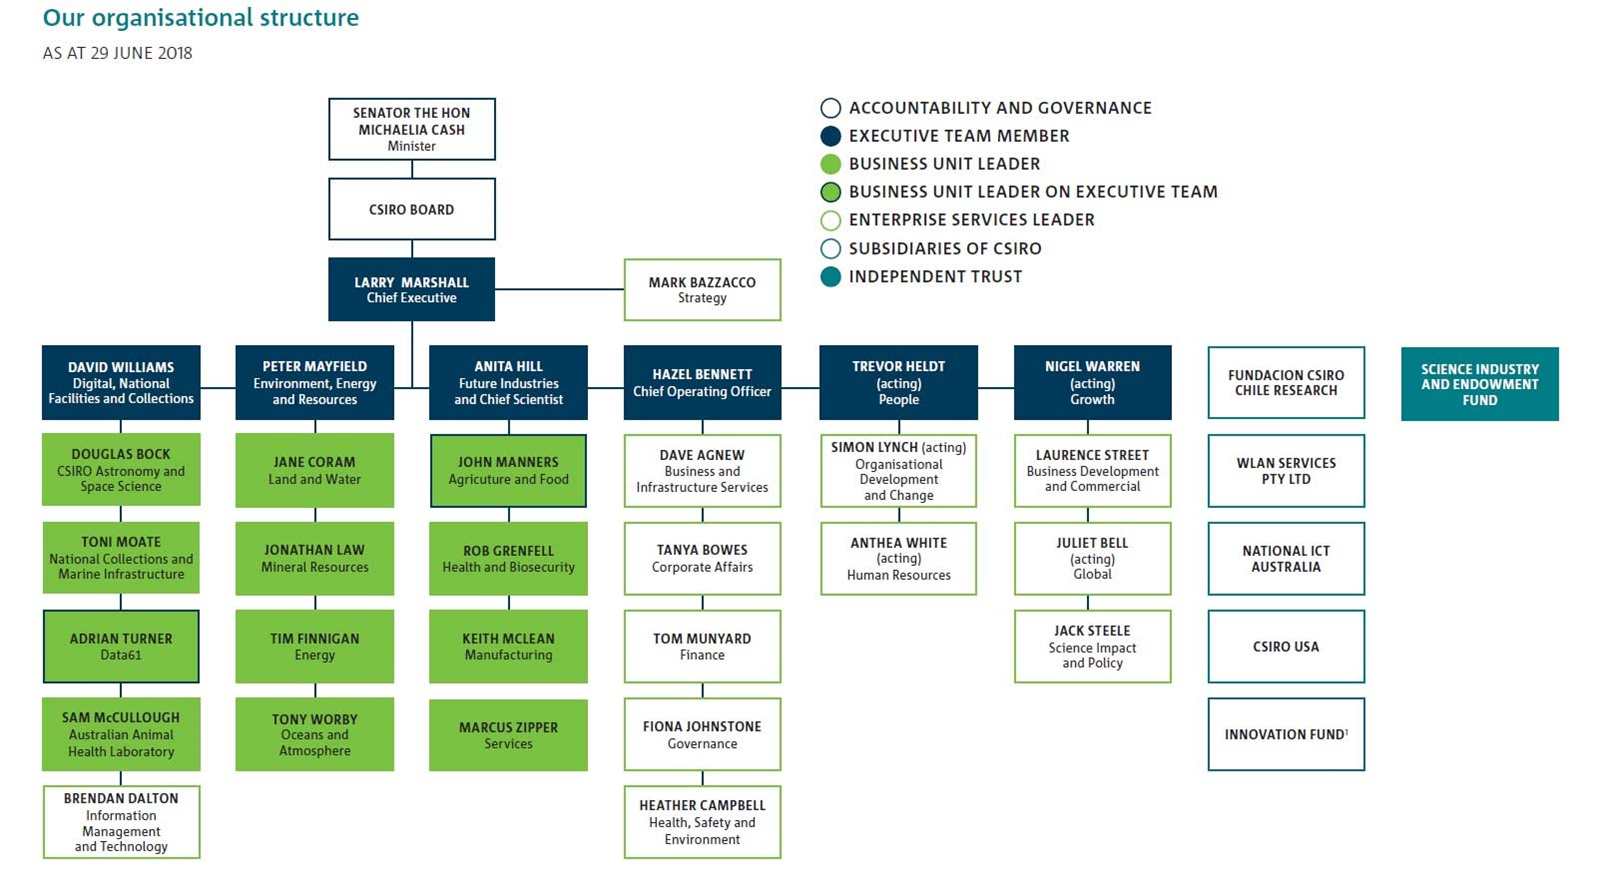
\includegraphics[width=16cm]{figures/csiro_struct.jpg}
    \caption{CSIRO Organizational Structure}\vspace{-4mm}
\end{figure}

\subsection{Areas of Interest}

\paragraph{}
DATA61 strives to build Australia's data driven future. Their programs can be divided into Analytics, Cyber-Physical Systems, Consumer Data Standards, Decision Sciences, Software and Computation Systems and Engineering and User Experience Design. Some of their key projects are:

\subsubsection*{Emesent - Hovermap}
\paragraph{}
Emesent is a spin-off company from the highly successful Hovermap project of DATA61. It is a state-of-the-art LiDAR based SLAM system to be fixed on industrial drones. Hovermap is also industrially used to analyze the structure and composition of various mineral deposits in rock cliffs, map underground mines and caves and used in forensics to analyze crime scenes.

\subsubsection*{SLAM}
\paragraph{}
DATA61 is a world leader in research, commercialization and impact of 3D LiDAR based simultaneous localization and mapping (3D SLAM). Their 3D SLAM algorithms and software is used to create highly accurate 3D maps of natural and artificial indoor and outdoor environments. This has been industrially used by the Australian Police to record homicide crime scenes, mapping caves, dinosaur footprints, record fragile cultural heritage sites and so on.

\subsubsection*{Legged Robots}
\paragraph{}
They have been focusing on Legged Robots since 2012. Modelled after insects, these six-legged and eight-legged robots can be used to navigate a disaster site and save lives. Several algorithms are being developed to address problems in legged navigation in complex environments.


\subsection{DARPA Subterranean Challenge}
\label{ssec:darpa}
\paragraph{}
The RAG of CSIRO was recently selected as one of the six funded teams worldwide for the DARPA Subterranean Challenge by United States Department of Defense. Therefore the next four years of research in Robotics in CSIRO will be more focused on developing robots that can simultaneously map and navigate complex environments such as underground tunnels, caves and mines without GPS or reliable communication with humans. It is an ideal project for DATA61, where their experience and expertise in SLAM, Hovermap and legged robots come together. By investing in this project for the next few years, DATA61 aims to develop new technology that can be later commercialized into different applications. 

%Image: Darpa challenge
\begin{figure}[H]
    \centering
    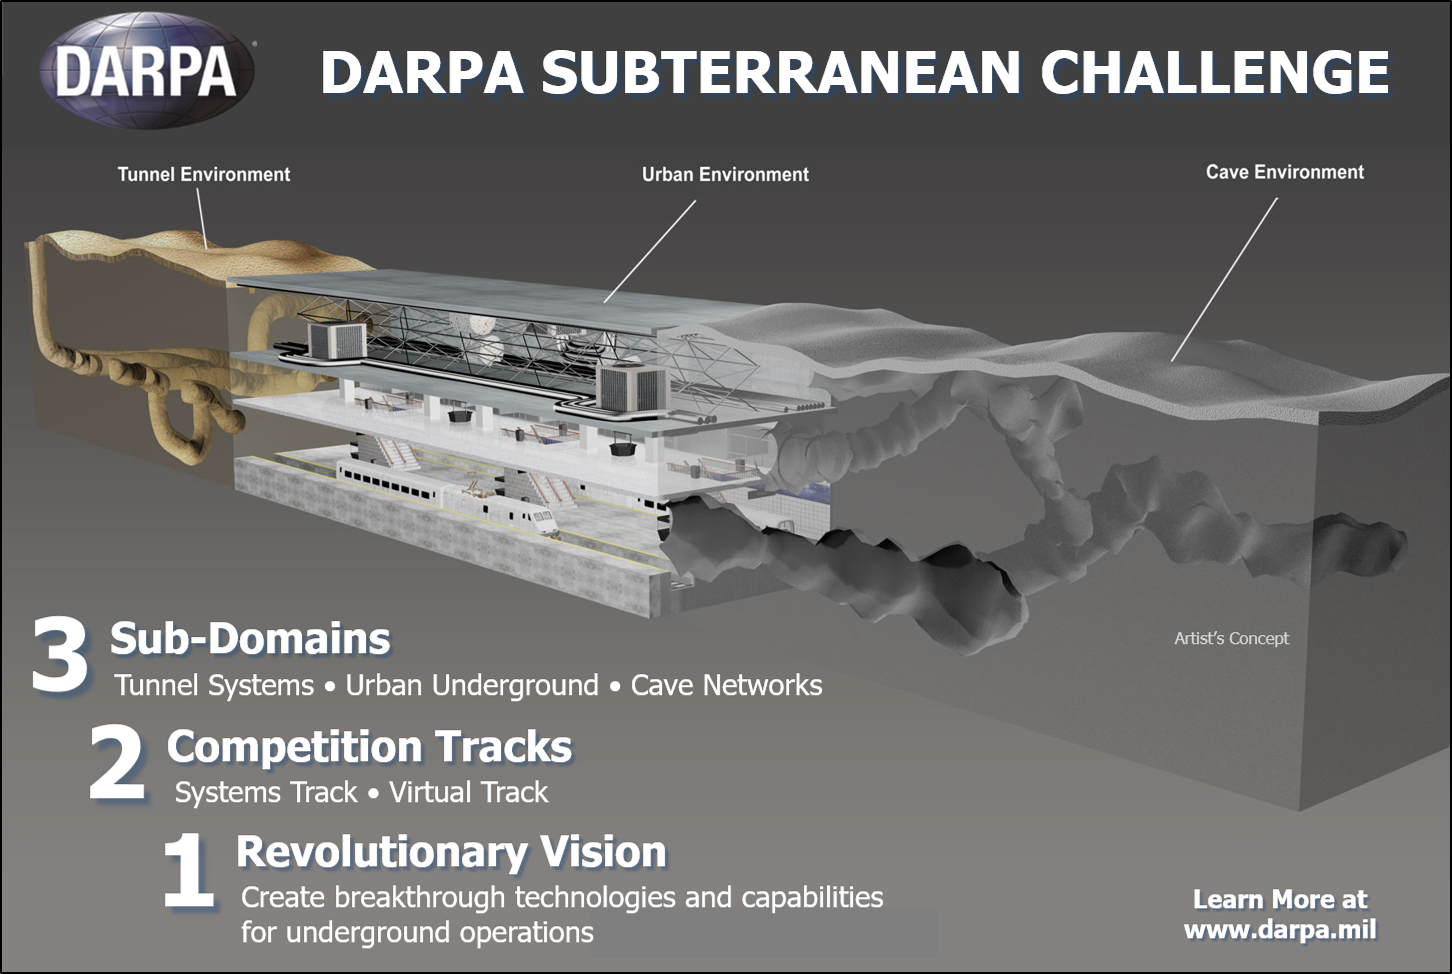
\includegraphics
        [width=12cm]
        {figures/subt_challenge.png}
    \caption{CSIRO focuses on DARPA challenge}\vspace{-4mm}
\end{figure}

\paragraph{}
This is the second competition held by DARPA to encourage development of cutting edge technology around the world. The first DARPA Robotics Challenge was held from 2012-2015 where the goal was to build a robot that can navigate a disaster site and perform tasks like driving a car, opening a door, drilling into the wall and so on, with an unreliable communications connection with the controlling humans. In case of future disasters like Fukushima Nuclear disaster, where humans cannot approach the site due to radiation, such robots can be utilized. The second competition focuses on subterranean environment, with the goal of buildings robots that can navigate the drug trafficking, human trafficking tunnels and save people stuck in mines and underground caves.

\paragraph{}
For this task, incorporating machine learning into the workflow of algorithm development and testing is of paramount importance for all researches in RAG. I addressed this problem by developing an efficient end-to-end pipeline for this and demonstrating it through two projects.


\subsection{Current Situation}
\paragraph{}
After years of research, development and commercialization of projects, DATA61 has risen as a world leader in many of their technologies. Hundreds of papers have been published from DATA61 in the past and are being published into reputed journals. Currently, DATA61 is being restructured and some of the technologies developed there have evolved into successful startup companies.

\subsection{Impacts on Sri Lankan Industry}
\paragraph{}
Being a part of the national research institute of Australia, DATA61 does not directly contribute to the Sri Lankan industry. However the research that is published in public domain can be used by Sri Lankan companies for their research and development.

\newpage
\subsection{SWOT Analysis}

\subsubsection*{Strengths}
\paragraph{}
DATA61 has ample resources and funds for its research programs. As a result a multitude of projects are being executed. Also the work culture in CSIRO encourages cross pollination of ideas and creativity. Their inclusive policy allows students and researchers from all around the world to come together and share their expertise and experience.

\subsubsection*{Weaknesses}
\paragraph{}
Although almost all researchers are friendly and helpful to each other, due to the way projects are assigned and due to the management structure, most of them work alone on a project. This has led to fragmentation, where people working on similar projects are unable to cooperate better. This is now addressed through weekly group meetings for Robotics, Machine Learning and standardization of the workflow, hardware and software APIs used in different projects.


\subsubsection*{Opportunities}
\paragraph{}
Being recognized as the world leader in their technologies, DATA61 has the opportunities to collaborate with other world class research institutes such as NASA Jet Propulsion Laboratory and ETH. We had the chance to attend lectures and discussions done by researchers from these institutes during our internship period. Also, DATA61 attracts talent from around the world and from within Australia, which would help them in the future research.

\subsubsection*{Threats}
\paragraph{}
DATA61 is a research organization that is funded for research that empowers the Australian industries. However, in the meanwhile they need to invest in pure science research the outcomes of which cannot be known in advance. This balance of funding projects of pure and applied science is vital to the success of DATA61 as an organization. If most of its research does not produce marketable technology, DATA61 is in danger of being under-funded by the australian government, meanwhile focusing more into applied science is not a sustainable strategy. This issue was discussed on multiple meetings as a part of their restructuring process.


\subsection{Usefulness to the Country}
\paragraph{}
DATA61 and CSIRO are important pillars of the Australian economy and society. The technologies materialized in DATA61 have laid the foundations for many companies in their industry and several companies collaborate with DATA61, paying them to use their service. This creates a win-win equilibrium that is beneficial to all parts of the economy.

\paragraph{}
Also, their research in healthcare, data privacy and infrastructure has been helping the australian society for the past few years. Their research into livestock management using IOT is helping the agriculture-based economy of the Queensland state. Hovermap and their research in mining is used to find new mineral deposits and analyze their composition. DATA61 is also modelling and devising algorithms to control traffic in different cities of Australia. 

\subsection{Suggestions to Improve the Company}
\begin{itemize}
    \item Implement a better project management system for intern students.
    \item Assign supervisors and well-defined projects that are compatible with the skills of students.
    \item Set deadlines for the student interns and monitor the progress.
    \item Provide concessions for students who live far away, as the public transport is considerably expensive.
\end{itemize}